%% Elsevier LaTeX submission.
%% Target: Knowledge-Based Systems (KBS), Elsevier.
%%
%% GENERATED FILE -- do not edit by hand.
%%   Source:    paper-kais/main.tex
%%   Generator: scripts/make_kbs_from_kais.py
%% The KAIS manuscript is the single source of prose and numbers. Edit that
%% file and regenerate, or the two submissions will drift apart, which is
%% exactly what happened to the previous hand-maintained copy.
%%
%% Build:  pdflatex main && bibtex main && pdflatex main && pdflatex main
\documentclass[final,5p,times,twocolumn]{elsarticle}

\usepackage{amsmath}
\usepackage{amssymb}
\usepackage{amsthm}
\usepackage{graphicx}
\usepackage{multirow}
\usepackage{array}
\usepackage{tabularx}
\usepackage{booktabs}
\usepackage{algorithm}
\usepackage{algpseudocode}
\usepackage{microtype}
\usepackage{xurl}
\usepackage[hidelinks]{hyperref}
\usepackage{tikz}
\usetikzlibrary{arrows.meta,positioning,fit,backgrounds,calc,shapes.geometric}
\graphicspath{{figures/}}

\hypersetup{hypertexnames=false,bookmarksdepth=3}

%% Figure 1 renders as live TikZ. Set \tikzfigurefalse to fall back to the
%% pre-rendered raster in figures/Fig1.png. This \newif MUST precede the
%% figure: without it \iftikzfigure is an undefined control sequence and the
%% compile dies inside the float.
\newif\iftikzfigure
\tikzfiguretrue

%% Explicit figure lettering sizes keep the diagrams legible and independent
%% of the document class's relative-size definitions.
\newcommand{\snFigMain}{\fontsize{9}{10.5}\selectfont}
\newcommand{\snFigSub}{\fontsize{8}{9.5}\selectfont}

\tikzset{
  snstage/.style={
    rectangle, draw=black, line width=0.65pt, fill=white,
    minimum height=18mm, inner sep=3pt, align=center,
    font=\snFigMain, text width=25mm},
  snstagekey/.style={
    rectangle, draw=black, line width=1.0pt, fill=white,
    minimum height=18mm, inner sep=3pt, align=center,
    font=\snFigMain, text width=25mm},
  snfold/.style={
    rectangle, draw=black, dashed, line width=0.5pt, fill=white,
    inner sep=2pt, align=center, font=\snFigSub, text width=22mm},
  snflow/.style={-{Stealth[length=4.5pt,width=3.5pt]}, draw=black,
    line width=0.75pt},
  sndata/.style={-{Stealth[length=4.5pt,width=3.5pt]}, draw=black,
    line width=0.5pt, dashed},
  snout/.style={
    rectangle, draw=black, line width=0.65pt, fill=white,
    minimum height=14mm, inner sep=3pt, align=center,
    font=\snFigMain, text width=34mm},
  sncredit/.style={snout},
  snremoval/.style={snout},
  sninteraction/.style={snout},
  snbranch/.style={draw=black, line width=0.65pt},
  snlbl/.style={font=\snFigSub, inner sep=1.2pt, text=black},
}

\renewcommand{\topfraction}{0.9}
\renewcommand{\bottomfraction}{0.8}
\renewcommand{\textfraction}{0.07}
\renewcommand{\floatpagefraction}{0.6}
\setcounter{topnumber}{3}
\setcounter{bottomnumber}{2}
\setcounter{totalnumber}{5}
%% placeins without [section]: a \FloatBarrier at every section head
%% forces a flush that reads as a gap before the heading. \FloatBarrier
%% remains available where a barrier is genuinely wanted.
%% Two-column floats: starred floats obey the \dbltop* parameters,
%% and 11 of 12 body floats here are starred.
\renewcommand{\dbltopfraction}{0.9}
\renewcommand{\dblfloatpagefraction}{0.6}
\setcounter{dbltopnumber}{3}
\usepackage{placeins}

\theoremstyle{plain}
\newtheorem{theorem}{Theorem}
\newtheorem{proposition}[theorem]{Proposition}
\newtheorem{lemma}[theorem]{Lemma}

\theoremstyle{definition}
\newtheorem{property}{Property}
\newtheorem{remark}{Remark}

%% \flushbottom, not \raggedbottom: in two columns ragged bottoms
%% leave slack at the foot of BOTH columns on every page.
\flushbottom
\emergencystretch=0.75em

\newcommand{\G}{\mathcal{G}}
\newcommand{\Cu}{C_u}
\newcommand{\Ueval}{\mathcal{U}_{\mathrm{eval}}}
\newcommand{\NDCG}{\mathrm{NDCG@10}}
\newcommand{\NDCGat}[1]{\mathrm{NDCG@}#1}
\newcommand{\LOOr}{\mathrm{LOO}_{\mathrm{rank}}}
\newcommand{\LOOe}{\mathrm{LOO}_{\mathrm{e2e}}}
\newcommand{\LOO}{\mathrm{LOO}}
\newcommand{\runint}[2]{%
  \shortstack{$#1$\\[-1pt]{\footnotesize $#2$}}}

\journal{Knowledge-Based Systems}
\biboptions{sort&compress}

\begin{document}

\begin{frontmatter}

\title{SignalShap: Exact Ranking-Stage Source Attribution for Hybrid
Recommenders}

\author[ensias]{Mouad Louhichi\corref{cor1}\fnref{orcid1}}
\ead{mouad_louhichi@um5.ac.ma}
\author[ensias]{Redwane Nesmaoui}
\ead{redwane.nesmaoui@um5.ac.ma}
\author[ensias]{Mohamed Lazaar}
\ead{mohamed.lazaar@ensias.um5.ac.ma}

\cortext[cor1]{Corresponding author.}
\fntext[orcid1]{ORCID: 0000-0002-6849-230X.}
\address[ensias]{National Higher School of Computer Science and Systems
Analysis (ENSIAS), Mohammed V University in Rabat, Rabat, Morocco}

\begin{abstract}
Ablation and Shapley attribution answer different questions: the cost
of removing a source and the allocation of system value. Conflating them can
produce opposite source-level conclusions.

We formulate attribution in a five-source hybrid recommender as a cooperative
game over collaborative, content, popularity, recency and sequential signals.
The payoff is baseline-centred NDCG@10 on coalition-independent candidates,
with coalition-specific ridge heads fit on validation data and evaluated on
test data. Enumerating all 32 coalitions eliminates aggregation sampling error.
At 500 draws, the 95th-percentile permutation error is 3.27\% of the
grand-coalition value, exceeding the 2.22\% ten-seed spread and 1.93\%
materiality threshold.

On two of three timestamped corpora, Shapley and ranking-stage leave-one-out
(LOO) disagree in sign by a material margin. Across ten seeds per corpus,
ranking-stage LOO matches observed end-to-end removal-loss orderings more
closely (mean Kendall $\tau$: LOO $0.96$--$1.00$; Shapley
$0.20$--$0.80$) and identifies the source with the smallest observed removal
loss on 90--100\% of fits versus 0--50\%. MovieLens-1M clears a declared
$0.60$ recall gate; Amazon-VG clears it only in an $N_{\max}=1\,200$
sensitivity with unchanged signs and orderings; Gowalla is a relative stress
test ($\rho=0.501$). We claim credit allocation under a declared ranking-stage
game, not retirement guidance.
\end{abstract}

\begin{keyword}
hybrid recommender systems \sep Shapley value \sep leave-one-out ablation
\sep source attribution \sep two-stage ranking
\end{keyword}

\end{frontmatter}

\section{Introduction}\label{sec:intro}

Hybrid recommenders combine architecturally distinct
scorers~\citep{burke2002hybrid}. Two questions then arise: how should the
system's observed ranking quality be allocated among its sources, and what
changes when one source is removed? The first is an allocation question; the
second is an intervention question. They need not yield the same source-level
conclusion.

Removal is commonly studied by \emph{leave-one-out} (LOO) ablation: disable
one source and measure the metric change. The resulting contrast is valid for
the intervention actually implemented, and dependence among sources does not
make it ill-defined. It is not, however, an allocation. LOO evaluates one
marginal contribution against the grand coalition, whereas Shapley combines
all $2^{n-1}$ marginal contributions using coalition-size weights. When sources
are substitutable, grand-coalition removal can have little effect even though
their shared capability contributes substantially. In a two-stage recommender,
the intervention must also be named: ranking-stage removal can hold candidates
fixed, while end-to-end removal changes retrieval and ranking together.

Cooperative game theory supplies the allocation rule. The Shapley
value~\citep{shapley1953} is the unique allocation satisfying efficiency,
symmetry, the null-player property and additivity, and it evaluates each player
against every coalition. We define a five-player game over collaborative,
content, popularity, recency and sequential sources. Its payoff is
baseline-centred NDCG@10 on a candidate set fixed across coalitions, so every
$v(S)$ is evaluated over the same items. Five players give $2^5=32$ coalition
values, which we enumerate exhaustively; the aggregation therefore introduces
no sampling error. Section~\ref{sec:verification} shows why that exactness is
material rather than merely convenient.

Material sign disagreement appears on two of the three timestamped corpora.
On MovieLens-1M, collaborative filtering receives the second-largest Shapley
allocation even though its ranking-stage removal improves the metric. Its two
strongest substitutive interactions are with the sequential and popularity
signals (Section~\ref{sec:attribution}; ESM~S3), providing a concrete mechanism
for the disagreement. When we remove
each source from both retrieval and ranking, ranking-stage LOO tracks the
ordering of observed losses substantially more closely than Shapley across ten
seeds per corpus. This comparison confirms that Shapley is an allocation, not
a retirement estimator. Our claims are limited to credit allocation under a
declared game; we do not offer retirement guidance, causal identification,
off-policy evaluation, or a state-of-the-art accuracy claim. Attribution-derived fusion
weights produced no resolvable gain over a global head, a negative result
reported in ESM~S5.

\medskip\noindent\textbf{Contributions.}
\begin{itemize}
\item \textbf{C1 (construct).} A ranking-stage cooperative game over
architectural sources, with a coalition-independent candidate set, a per-user
baseline-centred NDCG@10 payoff, and exact enumeration at small $n$.
\item \textbf{C2 (primary, empirical).} On three timestamped hybrids, Shapley
allocation and ranking-stage LOO can disagree in sign by a material margin, and
ranking-stage LOO, not Shapley, is the quantity that tracks observed end-to-end
retirement cost. Section~\ref{sec:discussion} maps decisions to estimands.
\item \textbf{C3 (verification).} The aggregation is checked against known
constraints: six analytic games, duplicate-injection symmetry, efficiency,
additivity and the null player, together with a measurement of what sampling
would have cost.
\end{itemize}

\medskip\noindent We ask three questions. \textbf{RQ1:} does the implementation
satisfy the constraints of correct Shapley aggregation, and how large would
approximation error be? \textbf{RQ2:} do Shapley and ranking-stage LOO disagree
materially, and can substitutive interactions explain the observed cases?
\textbf{RQ3:} which quantity aligns more closely with observed end-to-end
retirement losses?

Section~\ref{sec:related} reviews related work and background.
Section~\ref{sec:methodology} defines the game, algorithm and protocol;
Section~\ref{sec:verification} verifies the aggregation; and
Section~\ref{sec:results} reports attribution and retirement. Sections
\ref{sec:discussion} and~\ref{sec:conclusion} discuss the implications and
conclude. The electronic supplementary material (ESM) accompanying this article contains
proofs, full configuration details and the robustness suite.

\section{Related work and background}\label{sec:related}

\subsection{Feature-level attribution versus source-level attribution}
SHAP~\citep{lundberg2017} unified additive feature attribution, with extensions
to trees~\citep{lundberg2020}, data valuation~\citep{ghorbani2019} and
federated contribution~\citep{wang2020federated}.
Surveys~\citep{covert2021explaining,rozemberczki2022shapley} note that
model-agnostic estimators commonly sample, because the coalition lattice is
exponential in the number of players, with exact procedures reserved for
structured model classes. SHAP, LIME~\citep{ribeiro2016} and Integrated
Gradients~\citep{sundararajan2017} all answer ``which input features moved this
prediction?''. We ask which architectural component earned the system's ranking
quality. The unit of attribution differs, the payoff is a ranking metric rather
than a scalar output, and the decision it informs is the allocation of system
value across subsystems. Because there are five such subsystems rather than
hundreds of features, the complete game is small enough to enumerate: that
difference in granularity is what makes exactness available at all.

\subsection{Component-level games and the parent phenomenon}
Closer to our unit of analysis is work attributing behaviour to \emph{model
components}. Neuron Shapley~\citep{ghorbani2020neuron} treats individual
neurons as players with a performance payoff; ensemble
games~\citep{rozemberczki2021ensemble} treat whole classifiers as players and
allocate ensemble accuracy among them; and related work attributes changes in
performance rather than individual
predictions~\citep{zhang2023performance,shah2024coar,bell2024lsspa}. Closest to
our result is~\citet{kim2026forecast}, who compare an all-subsets Shapley
measure against leave-one-model-out in ensemble forecasting and relate the
disagreement to overlap in member errors.

We state the consequence plainly: neither component-level performance
attribution nor the contrast between an allocation and a grand-coalition
marginal is new in itself. The phenomenon is known outside recommendation. Our
narrower contribution is to instantiate it as a ranking-stage source game in a
\emph{two-stage} recommender, where removing a player also changes retrieval
and therefore the item set over which the metric is computed, and to adjudicate
the disagreement against an \emph{observed} retirement cost rather than against
another attribution. Shapley attribution has also been applied without labels,
including our own earlier work pairing approximated values with
clustering~\citep{louhichi2025gametheory}; that setting differs on every axis
that matters here, since one can switch off a recommender source but not a
feature of a clustering.

\subsection{Explainable recommendation in the data-engineering literature}
A large recent body of work explains recommendations by reasoning over
knowledge-graph paths, and it appears predominantly in the data-engineering
venues. \citet{li2023rlpath} learn path-exploration policies by reinforcement
learning for sequential explainable recommendation, and
\citet{li2024counterfactual} replace attention weights with counterfactually
learned path weights, arguing that attention is optimised for accuracy and is
unstable across reproductions. Both explain \emph{why a particular item reached
a particular user}, attributing to entities and relations inside one
differentiable model. Our unit is different and complementary: we attribute a
system-level ranking metric to architecturally distinct scorers, none of which
shares a graph or a gradient with the others, and we ask which source earned
the system's quality rather than which path justified an item. That difference
is also why these methods are not usable as baselines here; the comparators
that do apply to our unit are the attribution rules compared in
Section~\ref{sec:rulecomparison}.

Recent surveys of the field~\citep{garapati2025recsysreview,papadakis2022cftaxonomy}
confirm that component-level credit in hybrid architectures is still assessed
almost entirely by ablation, which is the practice this paper qualifies.

\subsection{Shapley for ranking}
RankSHAP~\citep{chowdhury2025rankshap},
RankingSHAP~\citep{heuss2025rankingshap} and ShaRP~\citep{pliatsika2025sharp}
bring Shapley to ranked outputs, but they attribute to \emph{features} of a
fixed candidate list and estimate by sampling. Because our players participate
in retrieval, a coalition would otherwise rank a different item set, which is
precisely why the game is defined on a coalition-independent candidate set.

The same cooperative-game machinery underpins data pricing and valuation,
where the exponential cost of exact computation is the central obstacle and
sampling is therefore the norm~\citep{pei2022datapricing}. Our setting inverts
that trade-off: five architectural players make the lattice small enough to
enumerate, which is what lets us \emph{measure} approximation error rather than
assume it (Section~\ref{sec:verification}).

\citet{sundararajan2020many} show that different Shapley formulations answer
different questions, so an attribution is only interpretable relative to a
declared game. We declare ours in Section~\ref{sec:game} and treat the choice,
not the axioms, as the substantive commitment. Graph and gradient
explainers~\citep{ying2019gnnexplainer,luo2020pgexplainer} operate inside one
differentiable model and do not apply across five architecturally distinct
scorers with no shared graph.

Hybrid designs~\citep{burke2002hybrid} are still assessed component-wise by
ablation, which is the practice this paper qualifies. Offline ranking
evaluation is itself sensitive to protocol and exposure
bias~\citep{ji2023leakage}, which is why our applicability diagnostics are
declared in advance in Section~\ref{sec:preconditions}.

\begin{table*}[tp]
\caption{Core notation used throughout the article.}
\label{tab:notation}
\small
\begin{tabularx}{\textwidth}{@{}l>{\raggedright\arraybackslash}X
  l>{\raggedright\arraybackslash}X
  l>{\raggedright\arraybackslash}X@{}}
\toprule
Symbol & Definition & Symbol & Definition & Symbol & Definition \\
\midrule
$\G$ & Source set & $v(S)$ & Coalition value
  & $\varphi_g$ & Shapley allocation \\
$\LOOr(g)$ & Ranking removal & $\LOOe(g)$ & End-to-end removal
  & $N_{\max}$ & Candidate cap \\
$\Ueval$ & Evaluation users & $\rho$ & Retrievability ceiling
  & $\lambda$ & Ridge penalty \\
\bottomrule
\end{tabularx}
\end{table*}

\subsection{Background}\label{sec:background}

A cooperative game is a pair $(\G, v)$ with players $\G$, $|\G| = n$, and
$v : 2^{\G}\to\mathbb{R}$ with $v(\varnothing)=0$. Table~\ref{tab:notation}
collects the notation used in the analysis. The Shapley value
\begin{equation}
\varphi_g(v) = \sum_{S\subseteq\G\setminus\{g\}}
  \frac{|S|!\,(n-|S|-1)!}{n!}\bigl[v(S\cup\{g\})-v(S)\bigr]
\label{eq:shapley}
\end{equation}
is the unique allocation satisfying efficiency
($\sum_g \varphi_g = v(\G)$), symmetry, the null-player property and
additivity. Leave-one-out is the single term at $S = \G\setminus\{g\}$,
\begin{equation}
\LOO(g) = v(\G) - v(\G\setminus\{g\}),
\label{eq:loo}
\end{equation}
so LOO and Shapley coincide only when no coalition other than the grand one is
informative, that is when $v$ is additive.

\paragraph{Two leave-one-out estimands, kept distinct}
This distinction carries the paper's result, so we fix notation for it.
$\LOOr(g)$ removes $g$ from a \emph{fixed-candidate ranker} only, leaving the
candidate set and therefore the item set intact. $\LOOe(g)$ removes it from
retrieval and ranking together, so the surviving sources rebuild the pool; this
is the deployment intervention. The two are not interchangeable, and the gap
matters for what each can be used for: $\LOOe$ equals the observed removal loss
by construction, so it cannot be evaluated as a \emph{predictor} of that loss,
whereas $\LOOr$ can, and is far cheaper because it does not re-run retrieval.
Neither estimand is invalidated by dependence among sources; the intervention
cost is well defined for the interacting system being measured. What LOO cannot
do is allocate, and that is a statement about the estimand rather than about
its statistical quality.

\paragraph{Semivalues, interactions and the payoff}
Semivalues relax efficiency by replacing the weights in
Equation~(\ref{eq:shapley}) with a general coalition-size distribution. Banzhaf
weights all coalitions equally and the binomial family interpolates by a
parameter $q$; both are used as comparators in ESM~S3, where we also record
that the \emph{size-uniform} semivalue is algebraically identical to Shapley
and so is not an independent comparator. Pairwise interaction
indices~\citep{grabisch1999interaction} measure
whether two players behave substitutively or complementarily under the same
game. With exactly one relevant test item per user,
NDCG@10~\citep{jarvelin2002cumulated} reduces to
$1/\log_2(1+\mathrm{rank})$ when that item appears in the top ten and $0$
otherwise, so a coalition value is an average of per-user reciprocal-log gains
over a common item set.

\section{Methodology}\label{sec:methodology}

Figure~\ref{fig:workflow} summarises the workflow from source fitting through
the complete coalition game to the three reported diagnostics.

\begin{figure*}[tp]
\centering
\iftikzfigure
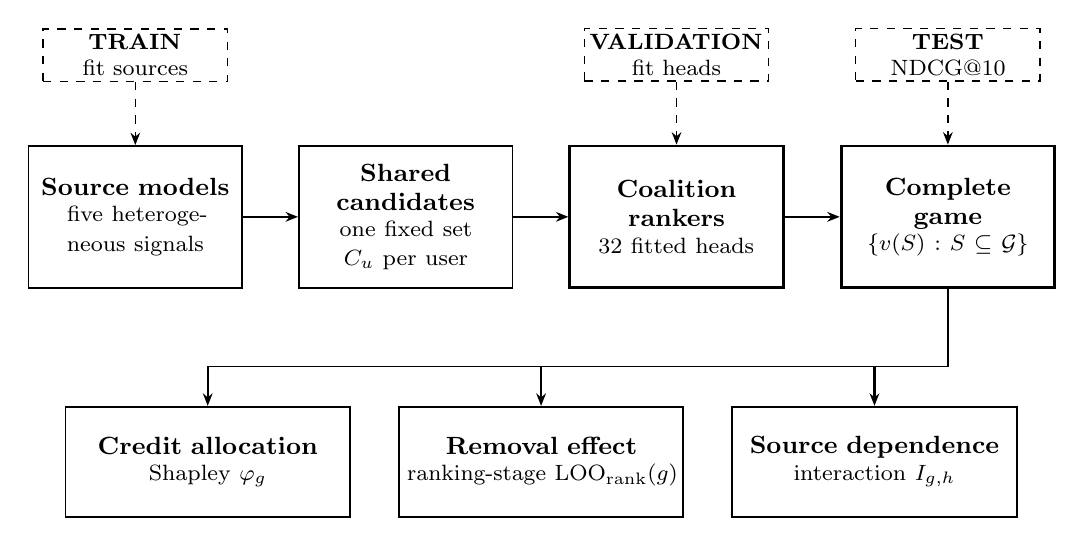
\begin{tikzpicture}[node distance=7mm]
\node[snstage] (src)
  {\textbf{Source models}\\[-1pt]
   {\snFigSub five heterogeneous signals}};
\node[snstage, right=of src] (cand)
  {\textbf{Shared candidates}\\[-1pt]
   {\snFigSub one fixed set $\Cu$ per user}};
\node[snstagekey, right=of cand] (heads)
  {\textbf{Coalition rankers}\\[-1pt]
   {\snFigSub $32$ fitted heads}};
\node[snstagekey, right=of heads] (game)
  {\textbf{Complete game}\\[-1pt]
   {\snFigSub $\{v(S):S\subseteq\G\}$}};

\draw[snflow] (src) -- (cand);
\draw[snflow] (cand) -- (heads);
\draw[snflow] (heads) -- (game);

\node[snfold, above=8mm of src] (train)
  {\textbf{TRAIN}\\{\snFigSub fit sources}};
\node[snfold, above=8mm of heads] (val)
  {\textbf{\mbox{VALIDATION}}\\{\snFigSub fit heads}};
\node[snfold, above=8mm of game] (test)
  {\textbf{TEST}\\{\snFigSub NDCG@10}};
\draw[sndata] (train) -- (src);
\draw[sndata] (val) -- (heads);
\draw[sndata] (test) -- (game);

\coordinate (outmid) at ($(cand)!0.5!(heads)$);
\node[snremoval, below=24mm of outmid] (removal)
  {\textbf{Removal effect}\\[-1pt]
   {\snFigSub ranking-stage $\LOOr(g)$}};
\node[sncredit, left=6mm of removal] (credit)
  {\textbf{Credit allocation}\\[-1pt]
   {\snFigSub Shapley $\varphi_g$}};
\node[sninteraction, right=6mm of removal] (interaction)
  {\textbf{Source dependence}\\[-1pt]
   {\snFigSub interaction $I_{g,h}$}};

\coordinate (busleft) at ($(credit.north)+(0,5mm)$);
\coordinate (busmid) at ($(removal.north)+(0,5mm)$);
\coordinate (busright) at ($(interaction.north)+(0,5mm)$);
\draw[snbranch] (game.south) |- (busmid);
\draw[snbranch] (busleft) -- (busright);
\draw[snflow] (busleft) -- (credit.north);
\draw[snflow] (busmid) -- (removal.north);
\draw[snflow] (busright) -- (interaction.north);

\end{tikzpicture}%
\else
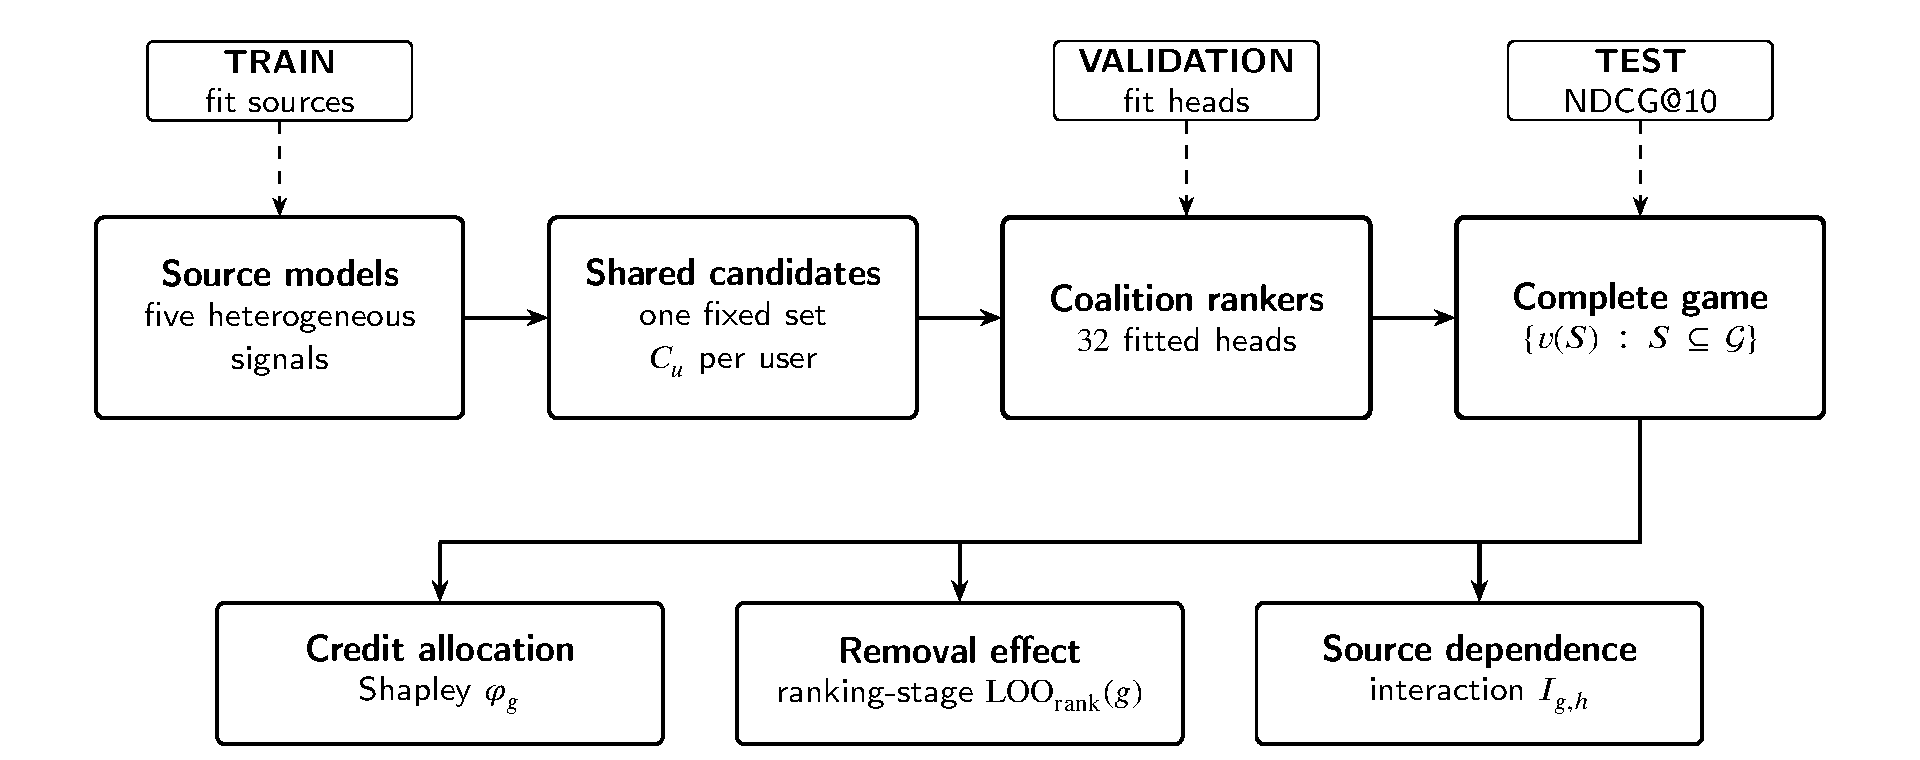
\includegraphics[width=\linewidth]{Fig1.png}
\fi
\caption{SignalShap workflow from source fitting and shared candidates to
exact-game diagnostics.}
\label{fig:workflow}
\end{figure*}

\subsection{The cooperative game}\label{sec:game}

The players are five source scorers, summarised in
Table~\ref{tab:sources}. Each maps a user $u$ and a candidate item $i$ to a
real score. We use deliberately simple, well-understood scorers: the paper is
about the attribution construct, not about the scorers, and we make no
state-of-the-art claim. We refer to the pipeline that fits these five sources,
enumerates the coalition lattice and aggregates as \emph{SignalShap}.

\begin{table*}[tp]
\caption{The five source scorers. Write $\mathcal{H}_u$ for user $u$'s training
history and $t_{\max}$ for the latest training timestamp. ``Declared overlap''
records substitutions predicted before the study was run, and which the
interaction indices later recovered in part.}
\label{tab:sources}
\small
\begin{tabularx}{\textwidth}{@{}llX@{}}
\toprule
Player & Signal & Scoring function $s_g(u,i)$, and declared overlap \\
\midrule
$cf$  & Collaborative
      & Implicit-feedback ALS~\citep{hu2008collaborative}, $64$ factors,
        confidence
        $c_{ui}=1+\alpha r_{ui}$ at $\alpha=1$, ridge
        $\lambda_{\mathrm{ALS}}=0.1$, $15$ iterations;
        $s_{cf}=x_u^\top y_i$. Declared to overlap $pop$. \\
\addlinespace[2pt]
$ct$  & Content
      & Cosine similarity in a $5\,000$-term L2-normalised TF--IDF space over
        item text: $p_u$ is the renormalised mean of consumed rows and
        $s_{ct}=p_u^\top M_i$. User-specific but time-invariant. Declared to
        overlap $rec$. \\
\addlinespace[2pt]
$pop$ & Popularity
      & Time-decayed global counts, half-life $h=180$ days:
        $s_{pop}=\log\bigl(1+\sum 2^{-(t_{\max}-t)/(86400h)}\bigr)$. Identical
        across users but not constant along a candidate row, so it survives
        $z$-normalisation. \\
\addlinespace[2pt]
$rec$ & Recency
      & Items assigned to one of $20$ clusters by argmax over a $20$-component
        SVD of a \emph{separate} $2\,000$-term TF--IDF matrix; $s_{rec}=
        2^{-(t_{\max}-\ell_{u\kappa(i)})/(86400\cdot30)}$ for the user's most
        recent interaction $\ell$ in that cluster, else $0$. \\
\addlinespace[2pt]
$seq$ & Co-occurrence
      & PPMI--SVD item embeddings~\citep{levy2014neural} (item2vec-style),
        pairs at distance $\le 5$,
        $64$ components; user vector is a recency-weighted mean of the last
        $5$ items with weights $0.8^k$. The co-occurrence matrix is
        \emph{symmetric}: order enters only through those weights, so this is
        not a sequential model in the SASRec sense, and the $cf$--$seq$
        interaction may partly reflect two collaborative signals. \\
\bottomrule
\end{tabularx}
\end{table*}

Every score is $z$-normalised per user over $\Cu$ before it enters the game.
That removes each source's location and positive linear scale, so the game is
invariant to positive affine rescaling of any source. It does \emph{not} make
only the ordering matter: the head fuses standardised columns linearly, so
relative spacing still affects the fused ranking, and a nonlinear monotone
transform of one source can change the result while preserving that source's
own ordering. Two implementation details are load-bearing for reproducibility.
The $rec$ argmax partition is not invariant to sign reversal of an SVD
component, so each component is canonicalised to a positive largest-magnitude
loading; this makes the partition a function of the data alone and $rec$
bit-identical across solver seeds. Where two singular values coincide, however,
the subspace has no preferred basis and the partition genuinely moves; that is
a property of the spectrum, not of the seed, and is the residual caveat for
$rec$.

\paragraph{A candidate set that does not depend on the coalition}
Every coalition is scored on one candidate set per user. Let $T_g(u,N_g)$ be
the first $N_g$ eligible items under the total order
$(-s_g(u,i),\,\text{item index})$, so that the item index breaks every score
tie including ties at the cutoff boundary. Then
\begin{equation}
\Cu \;=\; \operatorname{Trunc}_{N_{\max}^{(d)}}\!\Bigl(
  \bigcup_{g\in\G} T_g(u,N_g)\Bigr),
\qquad |\Cu| \le N_{\max}^{(d)},
\label{eq:candidates}
\end{equation}
where $d$ indexes the dataset, since the cap is frozen per corpus, and
$\operatorname{Trunc}_N$ retains the first $N$ items after sorting the union by
$\bigl(-\sum_{g\in\G} 1/\operatorname{rank}_g(i),\ \text{item index}\bigr)$,
with a source that did not retrieve $i$ contributing $0$. Sources begin at
equal depth $N_g = \lceil N_{\max}^{(d)}/|\G|\rceil$ and are deepened together
if the union underfills the cap. Both components of the truncation key are
invariant under permuting $\G$, so relabelling the players cannot change the
game. Writing $\Ueval = \{u : |\Cu| > 0\}$, users outside $\Ueval$ are excluded
from every coalition mean and reported separately as candidate-construction
failures.

This is the construct's load-bearing choice. If each coalition retrieved its
own pool, $v(S)$ and $v(S')$ would be NDCG values over different item sets and
their difference would confound ranking quality with retrieval coverage. The
alternative of a grand-coalition-only pool is not neutral either, and we
measured that cost rather than asserting it: under that design $\varphi_{ct}$
changes sign on MovieLens-1M. Three source-blind pool rules (ESM~S3) leave both
material disagreements intact. Oracle-pool recall equals $\rho$ exactly on
every corpus, in agreement with the dilution identity in
Equation~(\ref{eq:dilution}). Source scores enter the head $z$-normalised per
user over $\Cu$:
\begin{equation}
z_{u,g,i} =
\begin{cases}
\dfrac{s_g(u,i)-\mu_{u,g}}{\sigma_{u,g}}, & \sigma_{u,g}>0,\\[5pt]
0, & \sigma_{u,g}=0,
\end{cases}
\label{eq:z}
\end{equation}
so no source dominates through scale and a constant source row becomes zero.

\paragraph{Characteristic function}
For coalition $S$ we fit a ridge fusion head $w^{(S)}$ on \emph{validation}
data over the masked score matrix $Z^{(S)}_u$, and evaluate on \emph{test}
data:
\begin{equation}
v(S) \;=\; \frac{1}{|\Ueval|}\sum_{u\in\Ueval}
  \Bigl[\NDCG\bigl(\operatorname{rank}(Z^{(S)}_u w^{(S)}),\,
  \mathbf y^{\mathrm{te}}_u\bigr) - b_u\Bigr],
\label{eq:game}
\end{equation}
with $v(\varnothing)=0$ by construction. The ridge penalty $\lambda$ is frozen
before the study at a value selected on a MovieLens pilot; a sweep over eight
orders of magnitude appears in ESM~S3. For cutoff $K=10$, the per-user
baseline is the closed-form expectation
\begin{equation}
b_u =
\begin{cases}
\dfrac{1}{|C_u|}\displaystyle\sum_{r=1}^{\min(K,|C_u|)}
  \dfrac{1}{\log_2(r+1)}, & i_u^{\mathrm{te}}\in C_u,\\[7pt]
0, & i_u^{\mathrm{te}}\notin C_u,
\end{cases}
\label{eq:bu}
\end{equation}
the expected NDCG@10 of a uniformly random permutation of $C_u$, rather than a
sampled draw. Centring on an expectation removes a variance term that a single
random draw would inject into every coalition.

Equation~(\ref{eq:shapley}) is evaluated over all 32 coalitions with no
sampling. Exactness therefore qualifies \emph{the aggregation step, conditional
on the fitted characteristic function}, and nothing else: finite data,
stochastic fits, hyperparameter choices and floating-point libraries all remain
sources of error, and we quantify the first of these with ten-seed intervals
throughout. Source ordering does not matter: permuting the players changes no
value by more than $2.8\times10^{-5}$.

\subsection{Algorithm and cost}\label{sec:algorithm}

Algorithm~\ref{alg:signalshap} fits the sources once, builds $C_u$ once, then
sweeps the 32 coalitions. Two properties make the values comparable: every
coalition is scored on the same $C_u$, and every head is fit on validation
while every value is measured on test. Cost is dominated by scoring, not by the
game: the lattice contributes a factor of 32, and exact enumeration stays
practical to roughly $n \le 12$. Generative AI (OpenAI Codex) was used for code
scaffolding and consistency checking; every number reported here was recomputed
from the released commit.

\paragraph{The temporal state is frozen}
Sources are fitted on the training fold and not refreshed between the
validation and test steps, so the test step is a two-step-ahead forecast from a
frozen state rather than a one-step-ahead forecast with the validation event
folded in. This understates absolute performance, and we report the size of the
understatement rather than leaving it implicit: refreshing raises $v(\G)$ on
MovieLens-1M by $31.7\%$ $[+30.2\%,+33.1\%]$ over ten seeds, positive on
$10/10$, while preserving the ordering at $\tau = 1.00$ on every seed. The
sources whose values move are $seq$ ($+0.01393$) and $cf$ ($+0.00199$), both
sign-stable; $ct$ and $rec$ move by less than $10^{-4}$ with no stable sign
(ESM~S3). The choice is deliberate, since refreshing would give each coalition
a different information state and break comparability, but it is a limitation
on absolute magnitudes.

\paragraph{A retrievability ceiling on Gowalla}
Because held-out venues are masked if already seen in training, a fraction
$\rho$ of evaluated users cannot have their test item retrieved at all, and
contribute $v_u(S)=0$ for all 32 coalitions. The game then dilutes exactly,
\begin{equation}
v(S) \;=\; \rho \cdot v_{\mathrm{live}}(S),
\label{eq:dilution}
\end{equation}
verified to $1.4\times10^{-17}$ across all coalitions. On Gowalla
$\rho = 0.501$: half the users are exact zeros, all magnitudes are halved,
and orderings, signs, rank correlations and ratios are exactly invariant. The
practical consequence is stated plainly in Section~\ref{sec:preconditions}.

\begin{algorithm*}[t]
\caption{Exact ranking-stage SignalShap}\label{alg:signalshap}
\fontsize{8.5}{10}\selectfont
\begin{algorithmic}[1]
\Require train $\mathcal{D}_{\mathrm{tr}}$, validation $\mathcal{D}_{\mathrm{val}}$,
         test $\mathcal{D}_{\mathrm{te}}$; sources $\G$, $n=|\G|$; cap $N_{\max}$;
         growth limit $L=10$; penalty $\lambda$; cutoff $K$
\Ensure coalition values $v(S)$, source values $\varphi_g$, per-user $\varphi_g(u)$
\State fit every source $g \in \G$ on $\mathcal{D}_{\mathrm{tr}}$ only
\State score all eligible items per user from the TRAINING fold only; mask
       items seen in training \Comment{frozen-state protocol, see below}
\For{each user $u$}
  \State order each source list by descending score, then item index
  \State initialise $N_g\gets\lceil N_{\max}/n\rceil$ for every source
  \State grow $\bigcup_gT_g(u,N_g)$ as in Eq.~\eqref{eq:candidates}, stopping when
         $|C_u| \ge N_{\max}$, when every eligible per-source list is
         exhausted, or after $L$ passes; truncate by reciprocal-rank sum, then
         item index
  \If{$|C_u|=0$}
    \State record an empty-candidate diagnostic and continue
  \EndIf
  \State add $u$ to $\Ueval$
  \State $Z_u \in \mathbb{R}^{|C_u| \times n} \gets$ scores standardised by
         Eq.~\eqref{eq:z} \Comment{constant source rows become zero}
  \State $\mathbf{y}^{\mathrm{val}}_u, \mathbf{y}^{\mathrm{te}}_u \in \{0,1\}^{|C_u|}$
         $\gets$ indicators of the validation and test items
  \State $b_u \gets \dfrac{1}{|C_u|}\sum_{r=1}^{\min(K,|C_u|)}\dfrac{1}{\log_2(r+1)}$
         if the test item lies in $C_u$, else $0$
         \Comment{Equation~\ref{eq:bu}; deterministic, no permutation is drawn}
  \State \textbf{note} $i_u^{\mathrm{val}}$ is NOT added to the history and NOT
         masked before test scoring: one frozen source state serves both folds
  \State record whether validation equals test and whether the test item was
         observed in training
\EndFor
\State $A \gets \sum_{u\in\Ueval} |C_u|^{-1} Z_u^\top Z_u$, \quad
       $c \gets \sum_{u\in\Ueval} |C_u|^{-1} Z_u^\top \mathbf{y}^{\mathrm{val}}_u$
       \Comment{VALIDATION targets; accumulate once}
\For{each $S \subseteq \G$}
  \If{$S = \varnothing$}
    \State $v_u(S) \gets 0$ \ for all $u\in\Ueval$
           \Comment{$v(\varnothing) = 0$ exactly and per user}
  \Else
    \If{$\lambda > 0$}
      \State solve $\bigl[A_{SS} + \lambda I_{|S|}\bigr]w^{(S)}=c_S$
             \Comment{do not form an explicit inverse}
    \Else
      \State $w^{(S)} \gets A_{SS}^{+} c_S$
             \Comment{minimum-norm least squares; $A_{SS}$ is singular under
             exact duplicates. Singular values below
             $\varepsilon_{\mathrm{mach}}|S|\sigma_{\max}$ are truncated}
    \EndIf
    \State $v_u(S) \gets \NDCGat{K}\bigl(\mathrm{rank}(Z_u^{(S)} w^{(S)});\,
           \mathbf{y}^{\mathrm{te}}_u\bigr) - b_u$ \ for all $u\in\Ueval$
           \Comment{descending score, then item index; no tolerance relation}
  \EndIf
  \State $v(S) \gets |\Ueval|^{-1}\sum_{u\in\Ueval}v_u(S)$
\EndFor
\For{each $g \in \G$}
  \State $\varphi_g \gets \sum_{S \subseteq \G \setminus \{g\}}
         \tfrac{|S|!\,(n-|S|-1)!}{n!}\,[v(S \cup \{g\}) - v(S)]$
  \State $\varphi_g(u) \gets \sum_{S \subseteq \G \setminus \{g\}}
         \tfrac{|S|!\,(n-|S|-1)!}{n!}\,[v_u(S \cup \{g\}) - v_u(S)]$
\EndFor
\State verify efficiency $\sum_g \varphi_g = v(\G)$, the per-user decomposition,
       source-order invariance of $C_u$, and that no player is structurally
       degenerate according to Eq.~\eqref{eq:z}
\end{algorithmic}
\end{algorithm*}

\subsection{Formal properties}\label{sec:theory}

Efficiency holds by construction, so $\sum_g \varphi_g = v(\G)$ exactly. A
natural redundancy property, that a source duplicated into the system should
receive non-negative credit, is \emph{false} without monotonicity: we give a
three-player counterexample in ESM~S1 and record the corrected statement there
with its proof. This matters empirically rather than only formally, because all
three fitted games are non-monotone (Table~\ref{tab:preconditions}), so the
property does not apply on our data and negative $\varphi_g$ values are
faithful computations rather than implementation faults.

\subsection{Experimental setup}\label{sec:setup}

The five players are those of Table~\ref{tab:sources}. Before computing any
attribution we declared two expected substitutions, $cf$--$pop$ (popularity
leaking into implicit-feedback collaborative filtering) and $ct$--$rec$ (shared
content input), so that the interaction indices could be read against a
prediction rather than fitted to. Reference points include a uniform-weight
head, a popularity-only ranker, LightGCN~\citep{he2020lightgcn} and
SASRec~\citep{kang2018sasrec}; these are context for
absolute magnitudes and are deliberately under-tuned. They are not competitors
and no state-of-the-art claim is made or intended.

\paragraph{Corpora and protocol}
We use three timestamped corpora spanning a $36\times$ density range:
MovieLens-1M~\citep{harper2015movielens} ($6\,038$ users, $3\,533$ items), the
Video Games category of Amazon Reviews 2023~\citep{hou2026bridging}
($7\,120 \times 3\,516$), and Gowalla check-ins~\citep{cho2011friendship}
($8\,865 \times 82\,134$), each subsampled to fit the memory budget
(Table~\ref{tab:preconditions}). Timestamps are required, which is why these
three were chosen. Splits are per-user leave-last-out:
chronological within a user, which is standard for this protocol but not
globally time-blocked, so pooled training events postdate some users' held-out
events. We measured that rather than assuming it away: the mean fraction of a
user's training events that postdate their test event is $44\%$, $27\%$ and
$19\%$. A globally blocked replication on MovieLens-1M retains 526 of 6\,038
users and reproduces the paper's contrast, $\tau_{\LOOr} = 0.80$ against
$\tau_{\text{Shapley}} = 0.60$ with $\LOOr$ picking the correct source and Shapley
the wrong one, but does \emph{not} reproduce the per-source attributions:
under the blocked split the flip moves from $cf$ to $pop$ and $seq$. The
phenomenon replicates; the named sources do not. Ten seeds measure training
noise on fixed datasets, not a population of systems.

\paragraph{Reporting protocol}
Attribution and retirement results are reported over ten training seeds
(42--51). Brackets are run-to-run intervals
$\bar x \pm t_{0.975,9}\,s_x/\sqrt{10}$ and describe stochastic refitting on
fixed datasets. We are explicit that this is not population inference: ten
seeds bound training noise for these three corpora, and any statement about how
often the phenomenon occurs across hybrid recommenders in general would require
a sample of systems, which we do not have. Proportions carry Wilson intervals
rather than bare point estimates. A gap is called \emph{material} when it
exceeds $10^{-3}$ in absolute value, the same threshold applied to monotonicity
violations, and this threshold was fixed before the comparisons were run.

\subsection{Preconditions declared before the results}\label{sec:preconditions}

Two preconditions were declared before any attribution was computed, so that a
corpus could be disqualified on grounds independent of its results.

\emph{Monotonicity.} The redundancy argument of Section~\ref{sec:theory}
requires a monotone game. We therefore count violations
$v(S) > v(T)$ for $S \subset T$ on every fitted game rather than assume the
hypothesis. All three corpora violate it materially
(Table~\ref{tab:preconditions}), which is why the paper treats redundancy as an
interpretation rather than a theorem and why negative $\varphi_g$ values are
expected rather than anomalous.

\emph{Candidate recall.} Because the game is defined on a fixed pool, a test
item outside that pool is unreachable by every coalition and contributes zero
to all 32 values. Recall therefore bounds what the game can observe.

\begin{table*}[tp]
\caption{Corpus and candidate-set preconditions; monotonicity entries are
material/raw violation counts.}
\label{tab:preconditions}
%% \small: a ninth column (validation recall) was added in revision and the
%% widest row is 90 characters, close to the text block at normal size.
\small
\setlength{\tabcolsep}{3pt}
\begin{tabular*}{\textwidth}{@{\extracolsep{\fill}}lrrrrrrrl@{}}
\toprule
Corpus & Users / eval. & Items & Density & $N_{\max}$ & Recall & Val.\ & Monot. & \shortstack[l]{Prop.\\Sec.~\ref{sec:theory}} \\
 &  &  &  &  & (test) & recall & (mat./raw) &  \\
\midrule
MovieLens-1M & 6\,038 / 6\,035 & 3\,533  & $2.697\%$ & 600    & $0.748$ & $0.799$ & $7$ / $26$ & no \\
Amazon-VG    & 7\,120 / 7\,120 & 3\,516  & $0.469\%$ & 600    & $0.589^{\dagger}$ & $0.648$ & $4$ / $14$ & no \\
Gowalla      & 8\,865 / 8\,865 & 82\,134 & $0.075\%$ & 11\,623 & $0.450^{\dagger\ddagger}$ & $0.462$ & $6$ / $13$ & no \\
\bottomrule
\end{tabular*}
\par
\smallskip
\noindent\footnotesize $^{\dagger}$Below the $0.60$ gate; reported under the
ceiling restriction described in this section (relative contrasts only).
$^{\ddagger}$Recall on this corpus is bounded above by $\rho = 0.501$, the
fraction of users whose test venue is not already in their training history
(ESM Table~S9); $0.450$ is $0.898$ of that attainable ceiling and
the gate is unreachable at any $N_{\max}$. The corresponding ceilings are
$1.000$ for MovieLens-1M and $0.972$ for Amazon-VG. At $N_{\max}=1\,200$,
Amazon-VG test recall is $0.750$ and the attribution signs and orderings are
unchanged (ESM~S3).
\end{table*}

Candidate recall is an applicability diagnostic, not a quality metric, and the
$0.60$ gate was fixed before the runs. Only MovieLens-1M clears it in the
frozen configuration. Amazon-VG reaches $0.589$ at the frozen cap
$N_{\max}=600$ and $0.750$ at $N_{\max}=1\,200$, with the same qualitative
attribution at both, so we report it as gate-clearing only under the larger
cap. On Gowalla the ceiling of Equation~(\ref{eq:dilution}) bounds recall above
by $\rho = 0.501 < 0.60$, so the gate is unattainable at \emph{any} candidate
pool size and the corpus is retained as a relative stress test, for orderings
and signs rather than absolute magnitudes. Artefacts failing the gate are
admitted only via a declared exemption list and carry the restriction string
into every table built from them.

\section{Verifying the aggregation}\label{sec:verification}

Before interpreting any attribution we check the aggregation against
constraints whose answers are known independently of the data.

On observational data the correct allocation is unknown, so this section does
not validate real-system magnitudes. It checks whether the implementation
satisfies constraints fixed in advance.

\subsection{Known-answer games}
Six analytic games with closed-form Shapley vectors, spanning additive,
substitutive, complementary, null-player, harmful and unanimity structures, are
recovered with maximum absolute error $0$ (ESM Table~S1). The null-player and
harmful games matter most here: our fitted games are non-monotone and produce
negative $\varphi_g$, so it is necessary to establish that a negative value is
a faithful computation rather than an implementation artefact, and the harmful
game confirms that $-2$ is recovered exactly. Additivity, the remaining
uniqueness axiom that no other check exercises, holds to $4.4\times10^{-16}$.
Efficiency on the fitted corpora holds to machine precision.

\subsection{Duplicate injection}
Symmetry is checked on real data by injecting a near-duplicate of an existing
source at the level of raw scores, before any $z$-normalisation:
\begin{equation}
s_{g_{\mathrm{dup}}}(u,i) = s_g(u,i) + \eta\,\hat\sigma_g\,\epsilon_{u,i},
\qquad \epsilon_{u,i}\overset{\mathrm{i.i.d.}}{\sim}\mathcal N(0,1),
\label{eq:dup}
\end{equation}
with $g = cf$, $\hat\sigma_g$ one scalar per source over all eligible entries,
and the candidate set built \emph{before} injection and held fixed so that the
clone never enters retrieval and only the player set changes. At $\eta = 0$ the
original and the clone are exchangeable, so any rule satisfying symmetry must
give them equal value; ours does, to numerical precision. Ablation instead
assigns \emph{both} clones zero, since either alone is redundant given the
other. That is the substitutability failure of $\LOOr$ reproduced under a
controlled constraint rather than inferred from observational data. As $\eta$
grows the copy becomes noisier and $\LOOr$ becomes non-zero but erratic in sign.

\subsection{What exactness buys}
Calling the aggregation exact is only meaningful if sampling would have been
worse, so we measured it on the seed-42 MovieLens-1M ranking-stage,
baseline-centred NDCG@10 game. From its complete 32-coalition lattice we
estimated $\varphi$ by permutation sampling and by KernelSHAP at budgets
$M\in\{50,100,500,2000\}$ with 20 repeats each
(Figure~\ref{fig:sampling}). At $M=500$, permutation sampling still has a
95th-percentile error of $3.27\%$ of $v(\G)$, against a ten-seed spread of
$2.22\%$ and a materiality threshold of $1.93\%$; KernelSHAP is worse
throughout at this player count. Sampling error at a realistic budget is
therefore \emph{larger} than the effects this paper reports, and could
manufacture or erase a material sign flip. Exactness is load-bearing rather
than cosmetic.

\begin{figure*}[tp]
\centering
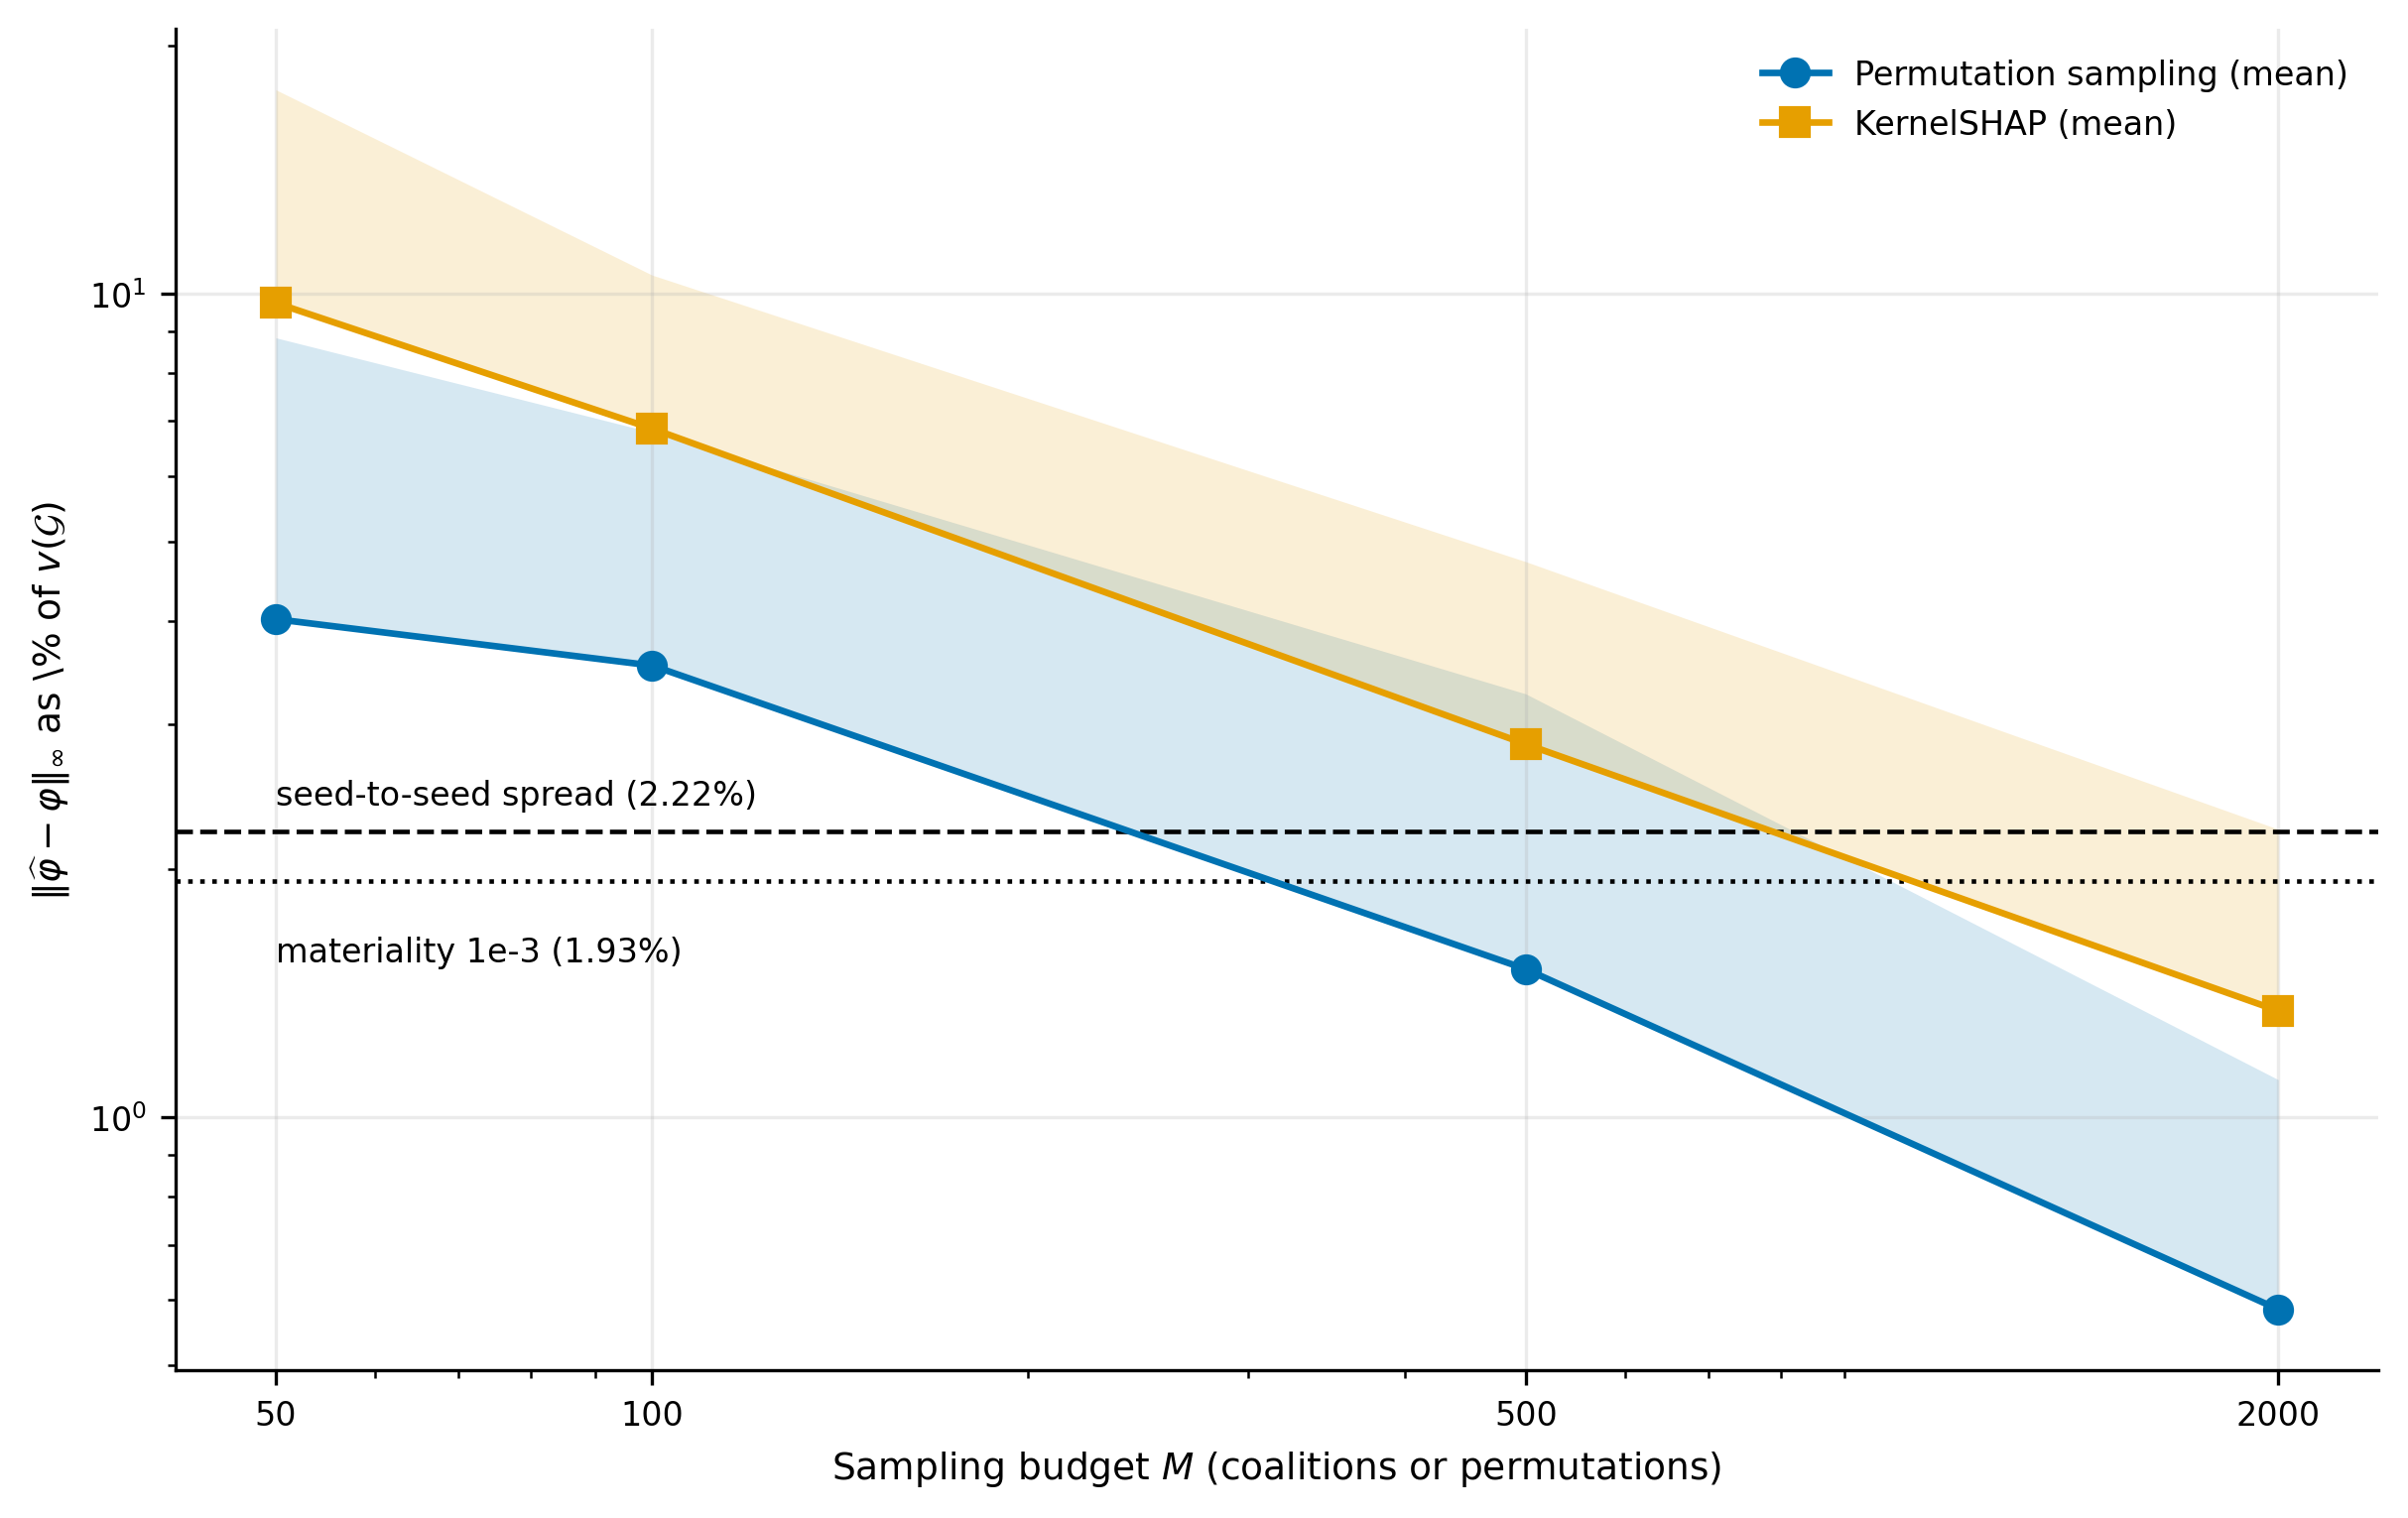
\includegraphics[width=0.86\textwidth]{Fig8.png}
\caption{Sampled Shapley error on the seed-42 MovieLens-1M ranking-stage,
baseline-centred NDCG@10 game, as a percentage of $v(\G)$, over 20 repeats per
budget; bands span the mean to the 95th percentile. Both reference lines are
quantities used in the paper: the ten-seed spread and the $10^{-3}$
materiality threshold. At $M=500$ the 95th-percentile permutation error remains
above both.}
\label{fig:sampling}
\end{figure*}

\subsection{Other values and interactions}
A comparator is informative only if it is genuinely a different member of the
semivalue family. The size-uniform weighting $p_k = 1/n$ is not: substituting
it returns Equation~(\ref{eq:shapley}) exactly, because
$|S|!\,(n-|S|-1)!/n! = 1/\bigl(n\binom{n-1}{|S|}\bigr)$, and it agrees to
exactly zero difference. We note this because the identity is easy to miss and
makes that particular comparison vacuous.

Among the genuine comparators, Banzhaf and two binomial semivalues rank the
sources identically to Shapley on MovieLens-1M. Robustness is not uniform
across corpora. On Gowalla all three agree with Shapley at $\tau = 0.80$, with
the $q = 0.25$ semivalue promoting $ct$ over $cf$ across a margin of only
$0.00037$ and Banzhaf transposing $pop$ and $rec$ across $0.00017$; these are
near-ties, not disagreements of substance. On Amazon-VG the disagreement is
stronger and we report it as a limitation rather than bury it: $\tau = 0.60$,
with Shapley leading on $cf$ and Banzhaf on $seq$. The ordering is therefore
robust to the coalition weighting on two corpora and not on the third.

Pairwise interaction indices recover part of the overlap declared in advance in
Table~\ref{tab:sources}. The two most negative pairs on MovieLens-1M are
$cf$--$seq$ at $-0.054$ and $cf$--$pop$ at $-0.025$, both substitutive, and
$cf$--$pop$ is one of the two declared overlaps. The recovery is partial rather
than complete, which is what we report. Full semivalue and interaction tables
are in ESM~S3.

\subsection{Which attribution rule predicts removal cost?}
\label{sec:rulecomparison}

Semivalues vary the coalition weighting but remain allocations, so comparing
them to one another cannot settle whether an allocation is the right instrument
for a removal decision. We therefore widen the comparison to the attribution
rules a practitioner would realistically reach for, and score each against the
same external criterion: the \emph{observed} end-to-end cost of retiring each
source. Every rule in Table~\ref{tab:rulecomparison} is a different linear
functional of the same 32 coalition values, so nothing is refitted and the
comparison adds no estimator variance. Beyond Shapley, Banzhaf and the binomial
semivalues, we include leave-one-in (the singleton value $v(\{g\})$, the rule
implied by scoring each source in isolation), exact forward-selection
importance averaged over all $n!$ greedy orders, and a uniform split
$v(\G)/n$ as a deliberately uninformative control.

\begin{table*}[tp]
\caption{Attribution rules scored against observed end-to-end retirement loss,
MovieLens-1M, seed 42. All rules are linear functionals of one 32-coalition
lattice, so no model is refitted. $\tau$ is Kendall agreement with the observed
loss ordering; ``picks'' is the source each rule nominates as having the
smallest removal loss, which is $cf$ in the observed data. The uniform split is
a constant vector, so its $\tau$ is undefined and it nominates nothing.}
\label{tab:rulecomparison}
\small
\begin{tabularx}{\textwidth}{@{}l
  >{\centering\arraybackslash}X
  >{\centering\arraybackslash}X
  >{\centering\arraybackslash}X
  >{\raggedright\arraybackslash}p{0.30\textwidth}@{}}
\toprule
Rule & $\tau$ vs.\ observed & Efficient & Picks & Character \\
\midrule
Ranking-stage LOO      & $+1.00$ & no  & $cf$  & grand-coalition marginal \\
Forward selection      & $+0.80$ & yes & $cf$  & greedy path, all orders \\
Binomial $q{=}0.75$    & $+0.40$ & no  & $rec$ & large coalitions weighted \\
Shapley                & $+0.20$ & yes & $ct$  & all coalitions, size weights \\
Banzhaf                & $+0.20$ & no  & $ct$  & all coalitions, uniform \\
Binomial $q{=}0.25$    & $+0.20$ & no  & $ct$  & small coalitions weighted \\
Leave-one-in           & $+0.20$ & no  & $ct$  & singleton value \\
Uniform split          & n/a     & yes & n/a   & uninformative control \\
\bottomrule
\end{tabularx}
\end{table*}

The ordering is the point. The two rules that track the removal outcome,
ranking-stage LOO and forward selection, are the two that condition on the
grand coalition or on a path towards it. Every rule that averages over all
coalitions, whatever its weighting, lands at $\tau = +0.20$ and nominates the
wrong source. The separation is therefore not an artefact of Shapley's
particular weights: it is a property of averaging over coalitions in which a
substitutable source has no substitute present, and Banzhaf, the binomial
semivalues and leave-one-in all inherit it. Notably, forward selection is
efficient \emph{and} predictive here, which shows the two properties are not
inherently in tension, though with $n = 5$ sources on one corpus we do not
claim that this generalises.

This is the comparison that supports the paper's claim. An allocation is not a
removal estimate, switching to a different allocation does not repair that, and
only changing the question does.

\section{Results}\label{sec:results}

\subsection{Allocation and removal disagree}\label{sec:attribution}

\begin{table*}[tp]
\caption{Ten-seed ranking-stage LOO and Shapley attribution. Brackets are
run-to-run intervals $\bar x \pm t_{0.975,9}\,s_x/\sqrt{10}$. The quantity
this paper contrasts is the paired gap $\Delta_g = \varphi_g - \LOOr(g)$, so it
carries its own interval, computed per seed and then aggregated rather than
differenced from the two marginal means; this is why the gap interval is not
the difference of the two columns beside it. ``Gap sign'' counts the fits on
which $\Delta_g$ keeps the sign of its mean. Fourteen of the fifteen cells are
unanimous; the exception is $rec$ on MovieLens-1M at $9/10$, whose gap is
$0.4\%$ of $v(\G)$ and which the paper does not interpret. Both material
disagreements have gap intervals excluding zero, at $38.8\%$ ($cf$,
MovieLens-1M) and $12.2\%$ ($pop$, Gowalla) of the respective $v(\G)$.}
\label{tab:loo}
\small
\setlength{\tabcolsep}{2.5pt}
\begin{tabular*}{\textwidth}{@{\extracolsep{\fill}}llrcrc@{}}
\toprule
Corpus & Source & $\LOOr$ & \shortstack{Shapley\\{\footnotesize [run interval]}}
       & \shortstack{Gap $\varphi_g-\LOOr$\\{\footnotesize [run interval]}} & Gap sign \\
\midrule
MovieLens-1M & $cf^{\dagger}$ & $-0.00457$ & \runint{+0.01573}{[+0.01542,+0.01604]} & \runint{+0.02030}{[+0.02007,+0.02053]} & $10/10$ \\
             & $ct^{\ddagger}$ & $+0.00052$ & \runint{-0.00016}{[-0.00024,-0.00008]} & \runint{-0.00068}{[-0.00088,-0.00047]} & $0/10$ \\
             & $pop$ & $+0.00070$ & \runint{+0.00643}{[+0.00638,+0.00649]} & \runint{+0.00573}{[+0.00551,+0.00596]} & $10/10$ \\
             & $rec$ & $+0.00010$ & \runint{+0.00032}{[+0.00022,+0.00042]} & \runint{+0.00022}{[+0.00003,+0.00040]} & $9/10$ \\
             & $seq$ & $+0.01745$ & \runint{+0.02993}{[+0.02963,+0.03024]} & \runint{+0.01249}{[+0.01209,+0.01288]} & $10/10$ \\
\midrule
Amazon-VG    & $cf$ & $+0.00890$ & \runint{+0.01980}{[+0.01937,+0.02022]} & \runint{+0.01089}{[+0.01062,+0.01117]} & $10/10$ \\
             & $ct$ & $+0.00011$ & \runint{+0.00195}{[+0.00183,+0.00207]} & \runint{+0.00183}{[+0.00165,+0.00201]} & $10/10$ \\
             & $pop$ & $+0.00394$ & \runint{+0.00178}{[+0.00166,+0.00190]} & \runint{-0.00216}{[-0.00244,-0.00188]} & $0/10$ \\
             & $rec^{\ddagger}$ & $+0.00014$ & \runint{-0.00049}{[-0.00053,-0.00046]} & \runint{-0.00063}{[-0.00069,-0.00057]} & $0/10$ \\
             & $seq$ & $+0.00761$ & \runint{+0.01883}{[+0.01865,+0.01900]} & \runint{+0.01122}{[+0.01107,+0.01138]} & $10/10$ \\
\midrule
Gowalla      & $cf$ & $+0.00743$ & \runint{+0.00711}{[+0.00698,+0.00725]} & \runint{-0.00032}{[-0.00039,-0.00025]} & $0/10$ \\
             & $ct$ & $+0.00547$ & \runint{+0.00678}{[+0.00672,+0.00683]} & \runint{+0.00131}{[+0.00121,+0.00141]} & $10/10$ \\
             & $pop^{\dagger}$ & $-0.00156$ & \runint{+0.00051}{[+0.00046,+0.00056]} & \runint{+0.00207}{[+0.00197,+0.00217]} & $10/10$ \\
             & $rec$ & $+0.00001$ & \runint{+0.00040}{[+0.00038,+0.00042]} & \runint{+0.00039}{[+0.00037,+0.00041]} & $10/10$ \\
             & $seq$ & $+0.00093$ & \runint{+0.00225}{[+0.00219,+0.00230]} & \runint{+0.00132}{[+0.00125,+0.00138]} & $10/10$ \\
\bottomrule
\end{tabular*}
\par\smallskip
{\raggedright\footnotesize $^{\dagger}$Material sign flip;
$^{\ddagger}$sign flip below the $10^{-3}$ materiality threshold.\par}
\end{table*}
\begin{figure}[tp]
\centering
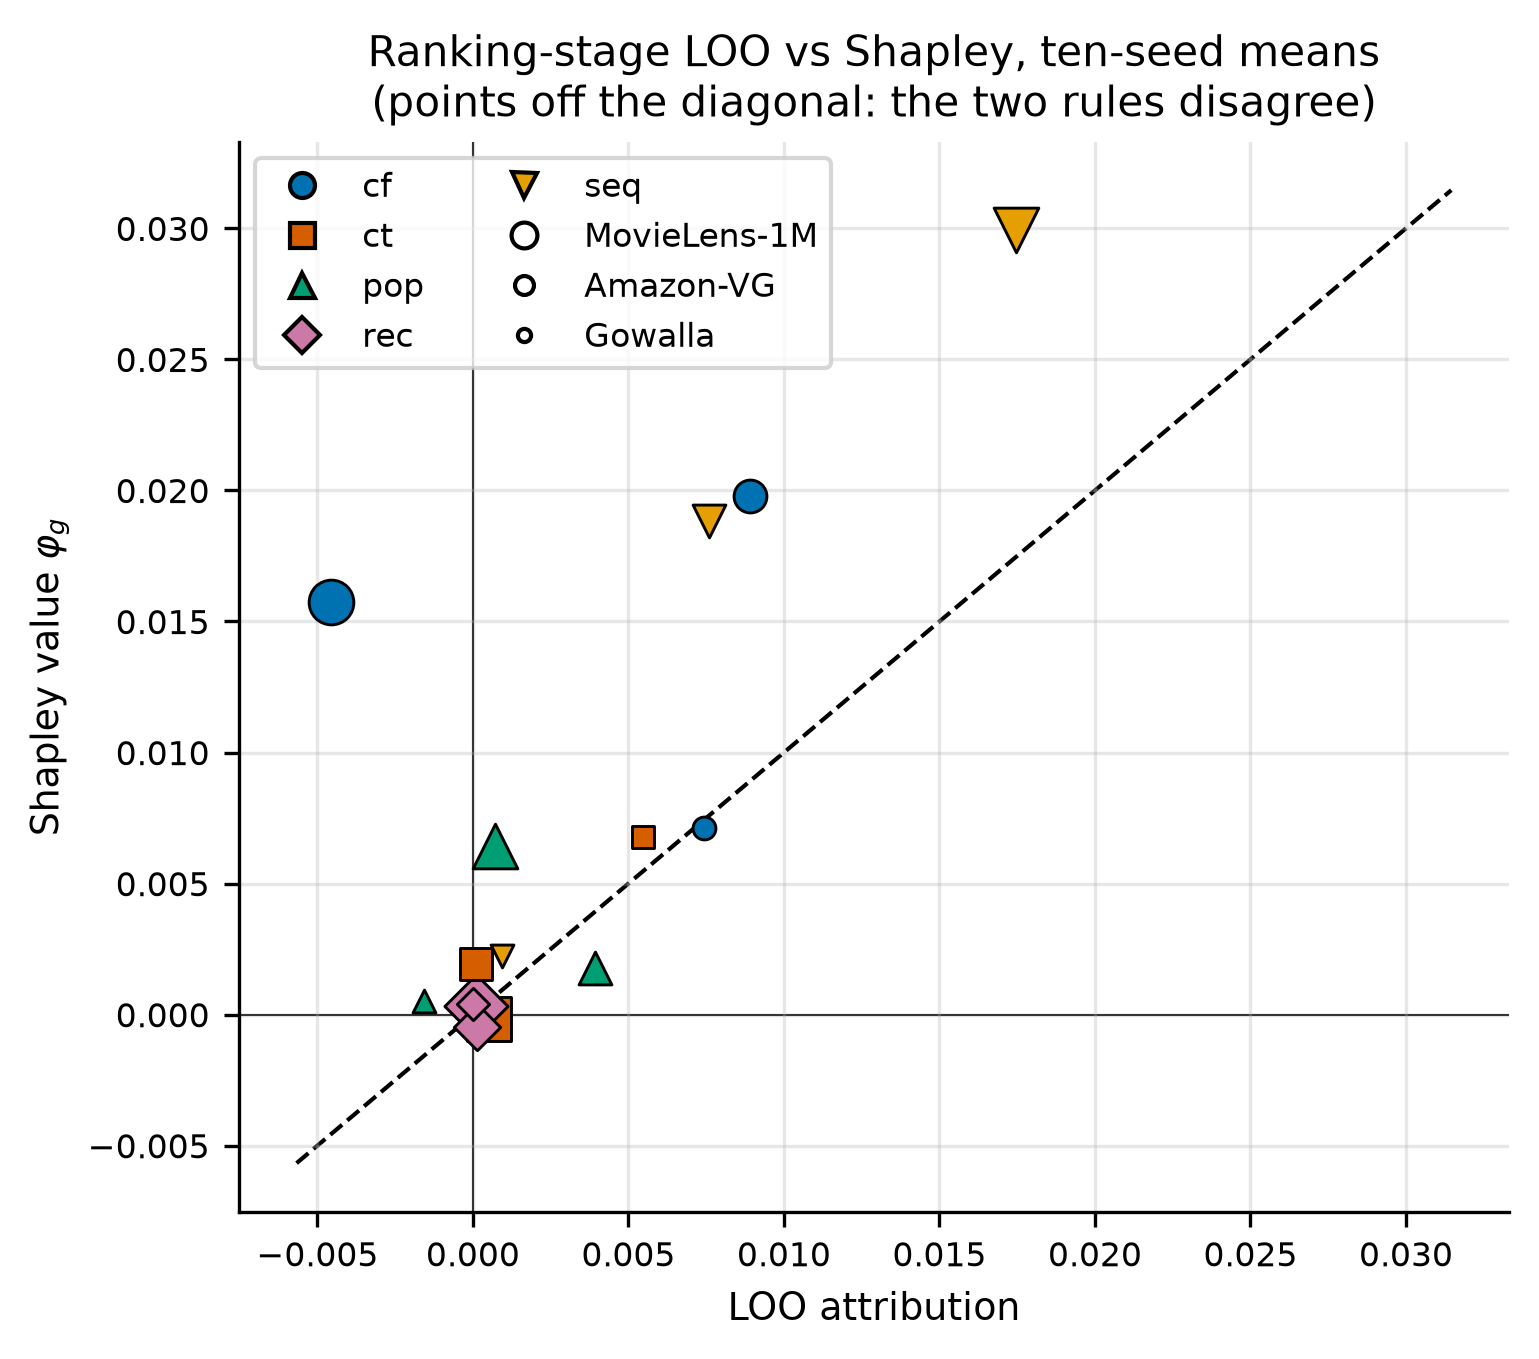
\includegraphics[width=\columnwidth]{Fig3.png}
\caption{Ten-seed mean Shapley versus ranking-stage LOO; the diagonal denotes
equality.}
\label{fig:scatter}
\end{figure}

Table~\ref{tab:loo} gives the per-source comparison over ten stochastic fits
and Figure~\ref{fig:scatter} plots it. Two of the three corpora contain a
\emph{material} sign disagreement, meaning one whose gap exceeds the $10^{-3}$
threshold we also apply to monotonicity.

On MovieLens-1M the source is $cf$. Shapley scores it $+0.01573$, the second
most valuable source in the system; $\LOOr$ scores it $-0.00457$, meaning its
removal \emph{improves} the fixed-candidate game. The paired gap is $+0.02030$
$[+0.02007,+0.02053]$, or $38.8\%$ of the ten-seed $v(\G) = 0.05225$, positive
on $10/10$ fits. On Gowalla the source is $pop$, with a gap of $+0.00207$
$[+0.00197,+0.00217]$, $12.2\%$ of $v(\G) = 0.01705$, again $10/10$: $\LOOr$ scores
the popularity signal negative where Shapley scores it positive. Because the
gap is a paired quantity it is computed per seed and then aggregated, which is
why its interval is not the difference of the two columns beside it.

Amazon-VG is a negative case and bounds the claim. Its only sign flip, on
$rec$, is $0.00063$, below the materiality threshold. The accurate statement is
therefore the weaker one: material sign disagreement occurs on two of the three
systems studied and is absent on the third. Three corpora cannot estimate how
common it is, and nothing in either rule announces in advance whether a given
system will exhibit it. Both material flips survive a $\lambda$ sweep over
eight orders of magnitude, three source-blind candidate pools, and score
perturbation at $\sigma\in\{0.1,0.5\}$ (ESM~S3).

\paragraph{Mechanism}
The account is \emph{qualitatively} the redundancy story, though formally
unavailable: all three fitted games are non-monotone, so the positivity
conclusion of Section~\ref{sec:theory} does not apply and what follows is
interpretation rather than theorem. A source whose signal is covered by others
costs little when removed from the \emph{grand} coalition, because the others
absorb its role, and ablation observes only that single contrast. Exact
enumeration averages the source's contribution over all $16$ coalitions in
which it can appear, including those where nothing covers for it, and so
recovers value the overlap conceals. On MovieLens-1M the collaborative signal
overlaps the sequential and popularity signals; on Gowalla it is the popularity
signal that is covered, by a geographic content signal essentially tied with
$cf$ at the top of the ranking ($0.00678$ against $0.00711$, an ordering that
resampling reverses).

The per-corpus orderings are
$seq \succ cf \succ pop \succ rec \succ ct$ (MovieLens-1M),
$cf \succ seq \succ ct \succ pop \succ rec$ (Amazon-VG) and
$cf \succ ct \succ seq \succ pop \succ rec$ (Gowalla, whose leading pair is
within $0.00033$ and exchanges under resampling). Pairwise Kendall $\tau$
between corpora is $0.40$, $0.20$ and $0.80$, none significant at $n = 5$
sources, so we make no cross-corpus consistency claim: identical near-zero
values from sources with no usable input would inflate such a comparison and
are not evidence of agreement.

\subsection{Which estimand predicts retirement cost?}\label{sec:retirement}

The sharper test is whether attribution predicts what removing a source
actually costs. We retired each source \emph{entirely}, from retrieval and
fusion alike, rebuilt candidates from the survivors, refitted, and measured the
observed end-to-end NDCG@10 loss. We write \emph{observed} rather than
\emph{true} throughout: this is one measured realisation under the reported
protocol, not a population quantity.

Two variants of the game bracket the design choice. Holding the deployed
grand-coalition head $w^{(\G)}$ fixed and merely masking it to $S$ gives
$v_{\mathrm{fixed}}$; letting each coalition retrieve its own $C_u(S)$ and
refit gives $v_{\mathrm{e2e}}$, under which coalition values are no longer
comparable across a fixed item set, which is exactly the property the main game
preserves. All three estimands are reported side by side in ESM Table~S10; their
orderings agree at $\tau \ge 0.80$ on both corpora where the comparison is
available.

\begin{table*}[tp]
\caption{MovieLens-1M retirement losses at seed 42; negative values indicate
improvement after removal.}
\label{tab:retirement}
%% tabular* + \extracolsep{\fill}: five narrow numeric columns have a small
%% natural width, so a plain tabular inside a full-width float leaves the
%% right-hand side of the span empty. This distributes the slack between the
%% columns instead.
\begin{tabular*}{\textwidth}{@{\extracolsep{\fill}}lrrrr@{}}
\toprule
Source & Observed loss & Recall after & Shapley & $\LOOr$ \\
\midrule
$cf$   & $-0.00468$ & $0.691$ & $+0.01538$ & $-0.00480$ \\
$rec$  & $-0.00128$ & $0.782$ & $+0.00053$ & $+0.00033$ \\
$ct$   & $-0.00050$ & $0.785$ & $+0.00002$ & $+0.00115$ \\
$pop$  & $+0.00253$ & $0.720$ & $+0.00648$ & $+0.00120$ \\
$seq$  & $+0.01702$ & $0.659$ & $+0.02927$ & $+0.01672$ \\
\midrule
\multicolumn{2}{@{}l}{Rank agreement with observed loss}
      & & $\tau = +0.20$ & $\tau = +1.00$ \\
\bottomrule
\end{tabular*}
\end{table*}
\begin{table*}[tp]
\caption{Ten-seed agreement with observed end-to-end retirement loss. Brackets
are run intervals for rank agreement and Wilson intervals for correct-source
rates. Paired $\Delta\tau=\tau_{\LOOr}-\tau_{\mathrm{Shapley}}$ is the effect
measure; $p_{\mathrm{Holm}}$ adjusts the three paired Wilcoxon
comparisons~\citep{wilcoxon1945individual,holm1979simple}.}
\label{tab:retire-seeds}
\small
\begin{tabularx}{\textwidth}{@{}l
  >{\centering\arraybackslash}X
  >{\centering\arraybackslash}X
  >{\centering\arraybackslash}X
  >{\centering\arraybackslash}p{0.11\textwidth}@{}}
\toprule
Corpus & $\tau_{\LOOr}$ & $\tau_{\mathrm{Shapley}}$
       & Paired $\Delta\tau$ & $p_{\mathrm{Holm}}$ \\
\midrule
MovieLens-1M & \runint{0.96}{[0.90,1.00]}
             & \runint{0.20}{[0.20,0.20]}
             & \runint{+0.76}{[+0.70,+0.80]} & $0.0059$ \\
Amazon-VG    & \runint{0.96}{[0.90,1.00]}
             & \runint{0.74}{[0.68,0.80]}
             & \runint{+0.22}{[+0.16,+0.28]} & $0.0059$ \\
Gowalla      & \runint{1.00}{[1.00,1.00]}
             & \runint{0.80}{[0.80,0.80]}
             & \runint{+0.20}{[+0.20,+0.20]} & $0.0059$ \\
\midrule
\multicolumn{5}{@{}l}{\textbf{Source with the smallest observed loss identified correctly [Wilson]}} \\
Corpus & \multicolumn{2}{c}{$\LOOr$ correct}
       & \multicolumn{2}{c}{Shapley correct} \\
\cmidrule(lr){1-1}\cmidrule(lr){2-3}\cmidrule(l){4-5}
MovieLens-1M & \multicolumn{2}{c}{$100\%\ [72,100]$}
             & \multicolumn{2}{c}{$0\%\ [0,28]$} \\
Amazon-VG    & \multicolumn{2}{c}{$90\%\ [60,98]$}
             & \multicolumn{2}{c}{$50\%\ [24,76]$} \\
Gowalla      & \multicolumn{2}{c}{$100\%\ [72,100]$}
             & \multicolumn{2}{c}{$0\%\ [0,28]$} \\
\bottomrule
\end{tabularx}
\end{table*}

The comparison is not tautological, and the reason is the distinction fixed in
Section~\ref{sec:background}. The ranking-stage LOO column of
Table~\ref{tab:retirement} is
$\LOOr$, computed on the same kind of fixed-candidate game as the Shapley
column. It is \emph{not} $\LOOe$, which equals the observed loss by
construction and so could not be evaluated as a predictor of it. The finding is
therefore informative: a quantity computable \emph{without} re-running
retrieval predicts the expensive end-to-end outcome, and predicts it far better
than the Shapley value of the same game.

On seed 42 (Table~\ref{tab:retirement}) $\LOOr$'s ranking matches the observed
loss exactly, $\tau = 1.00$ against Shapley's $0.20$ (exact two-sided
permutation $p = 0.017$ and $p = 0.82$ at $n = 5$ sources), and it identifies
$cf$ as the source with the smallest observed removal loss where Shapley
selects $ct$. Removing $cf$ improves the end-to-end metric by $0.00468$.

Over ten seeds (Table~\ref{tab:retire-seeds}) $\LOOr$'s mean rank agreement is
$0.96$, $0.96$ and $1.00$ against Shapley's $0.20$, $0.74$ and $0.80$. $\LOOr$
is not perfect on every seed, but across all thirty fits it is never worse:
29 wins and one tie. The practical gap is starker than the correlations: $\LOOr$
identifies the source with the smallest observed removal loss on $100\%$,
$90\%$ and $100\%$ of seeds against $0\%$, $50\%$ and $0\%$ for Shapley, so on
two of three corpora Shapley never once selects the right source to switch off.
Ten seeds bound these proportions loosely and we give Wilson intervals rather
than let point estimates stand: $100\%$ is $[72,100]$ and $0\%$ is $[0,28]$, so
the separation survives on MovieLens-1M and Gowalla while the Amazon contrast,
$[60,98]$ against $[24,76]$, overlaps. Pairing by seed, $\Delta\tau =
\tau_{\LOOr}-\tau_{\text{Shapley}}$ is $+0.76\ [+0.70,+0.80]$, $+0.22\
[+0.16,+0.28]$ and $+0.20$ with zero variance, no interval containing zero. We
read this as run-to-run stability of the contrast on fixed datasets, not as
population inference over hybrid recommenders.

The result is consistent with the theory rather than a contradiction of it.
Removing $cf$ improves end-to-end NDCG@10 by $0.00468$ while dropping candidate
recall from $0.748$ to $0.691$: the collaborative signal is substantially
substitutive with $seq$ and $pop$, the two most negative interaction pairs, so
inside the grand coalition its scores add noise the others already cover.
Shapley averages over coalitions in which $cf$ has no substitute and therefore
assigns the capability positive value \emph{under the declared game}. We say
this because no external ground truth for the allocation exists, and the two
statements describe different games.

\section{Discussion}\label{sec:discussion}

The two rules answer different questions, and Table~\ref{tab:decisions-kais}
maps each decision to the estimand that answers it. $\LOOe$ is definitionally
aligned with ``what happens in this offline protocol if I remove this one
source''. Shapley answers ``how should measured ranking quality be divided
among sources under the declared game''. We claim only the latter.

\begin{table*}[tp]
\caption{Decision-to-estimand mapping. The final row is the paper's own
boundary: the contrast between allocation and removal replicates under a
globally blocked split, while the identity of the flipping source does not.}
\label{tab:decisions-kais}
\small
\begin{tabularx}{\textwidth}{@{}lX@{}}
\toprule
Decision & Estimand that answers it \\
\midrule
Remove one source from the deployed system
  & $\LOOe$; $\LOOr$ tracks it closely here without re-running retrieval \\
Divide measured ranking utility among sources
  & Shapley on the declared game \\
Rank sources under other coalition weightings
  & Banzhaf or binomial semivalues, for ordering only \\
Decide where to invest engineering effort next
  & \emph{Not established.} Requires headroom, cost, latency and risk, none of
    which enter $v$ \\
Trust the named flipping source under a global time split
  & \emph{No.} Trust the allocation-versus-removal contrast: \emph{yes} \\
\bottomrule
\end{tabularx}
\end{table*}

\subsection{Interpreting source allocations}
A positive $\varphi_g$ licenses the statement that source $g$ is allocated
value under this game. It does not license keeping $g$, and a negative
$\varphi_g$ does not license dropping it; on MovieLens-1M the source with the
second-largest allocation is also the one whose removal improves the metric.
The allocation is descriptive, not prescriptive. In particular it is not a
guide to future engineering investment, which additionally depends on
improvement headroom, implementation cost, latency, maintenance burden and
deployment risk, none of which enter the characteristic function.

\subsection{Scope of the explainability claim}
The method explains a fitted system at the level of architectural sources. The
global values divide baseline-centred ranking utility and the per-user
decomposition is an exact identity, so faithfulness is defined relative to the
declared characteristic function and verified by the checks of
Section~\ref{sec:verification}. Interaction indices add information about
substitutive behaviour under that same game, but they are not causal redundancy
estimates. We did not evaluate whether end users understand or prefer these
explanations, and we do not establish seed stability of individual-user
attributions. The supported claim is system-diagnostic source attribution, not
human-facing explanation quality.

\subsection{Threats to validity}\label{sec:threats}

\emph{Construct.} The game is ranking-stage: it holds candidates fixed so that
coalition values are comparable, which is exactly why it is not the deployment
intervention. That gap is the paper's subject, not an oversight.
\emph{Internal.} Splits are per-user chronological rather than globally
blocked, with the leakage fractions quantified in Section~\ref{sec:setup}; the
blocked replication preserves the contrast but not the named sources.
\emph{Statistical.} Ten seeds describe training randomness on fixed datasets.
Intervals and paired tests are conditional on treating seeds as exchangeable
runs and are not population inference.
\emph{External.} Three corpora, five deliberately simple players, one
subsample per corpus. Gowalla's magnitudes are halved by the retrievability
ceiling, so only its orderings and signs are read. No causal or off-policy
claim is made, no fairness claim is made, and no state-of-the-art comparison is
intended: the neural components that appear in the supplement are reference
points, are under-tuned, and are not competitors.
\emph{Provenance.} The ten-seed attribution and retirement results are primary
and were regenerated under the final source-symmetric candidate rule. Several
labelled single-seed diagnostics predate that regeneration and are sensitivity
analyses rather than confirmatory evidence; on MovieLens-1M the two rules agree
to $\max_g|\Delta\varphi_g| = 2.8\times10^{-5}$ with identical ordering.
ESM Table~S4 lists which group is which, including the Gowalla diagnostics that
could not be regenerated because five dense $8\,865\times82\,134$ score
matrices exhausted memory.

\section{Conclusion}\label{sec:conclusion}

Source ablation and Shapley attribution answer different questions, and on two
of three timestamped hybrid recommenders they disagree in sign for at least one
source by a material margin. When each source is retired outright,
ranking-stage leave-one-out tracks the observed end-to-end cost and Shapley
does not: mean rank agreement $0.96$--$1.00$ against $0.20$--$0.80$, and the
source with the smallest observed removal loss identified on $90$--$100\%$ of
fits against $0$--$50\%$. Exact enumeration is what makes these comparisons
safe, since sampling at a realistic budget carries error larger than the
effects themselves.

The claim is bounded: we allocate credit in a declared ranking-stage game on
three corpora with five simple players under one offline protocol, and we do
not offer retirement guidance, causal identification, or a fusion method.
Future work: cost-aware characteristic functions that price latency and
maintenance; principled sampling beyond $n \approx 12$; graph-neural and
Transformer components as players rather than baselines; and a repeat-aware
protocol for check-in data, where the retrievability ceiling bites hardest.

\section*{CRediT authorship contribution statement}
\textbf{Mouad Louhichi:} Conceptualization, Methodology, Software, Formal
analysis, Investigation, Writing -- original draft, Visualization.
\textbf{Redwane Nesmaoui:} Software, Validation, Data curation, Writing --
review and editing. \textbf{Mohamed Lazaar:} Supervision, Methodology,
Resources, Writing -- review and editing.

\section*{Declaration of competing interest}
The authors declare that they have no known competing financial interests or
personal relationships that could have appeared to influence the work reported
in this paper.

\section*{Funding}
The authors declare that no funds, grants, or other support were received
during the preparation of this manuscript.

\section*{Ethics}
The study performs secondary analysis of previously released, de-identified
human-generated ratings, reviews, and check-ins under the dataset licenses
recorded in the artefact, and involves no new participant recruitment or
intervention. Geographic check-ins can retain re-identification risk even after
direct identifiers are removed; we use only aggregate geographic cells and
redistribute no event records. Popularity-based signals can reinforce exposure
disparities, and no fairness claim is made.

\section*{Data availability}
This work uses three public corpora and redistributes none of them.
MovieLens-1M is used under the GroupLens research-use license, Gowalla
check-ins come from the SNAP collection, and the Video Games category is taken
from the Amazon Reviews 2023 corpus; the fetch scripts in the repository
retrieve each from its original source. All derived data behind every reported
number is released with the code, together with \texttt{MANIFEST.json}, which
records a SHA-256 for each artefact file with the commit and environment that
produced it, including the BLAS backend. \texttt{PROVENANCE.md} maps every
table and figure to the artefact, platform, candidate rule and seeds behind it.
A reader reproducing from raw data must refetch the corpora first, and a run on
a different BLAS reproduces the reported signs and orderings but not every
fifth decimal.

\section*{Code availability}
The implementation, configuration files, and scripts required to reproduce the
reported experiments, tables, and figures are publicly available at
\url{https://github.com/mouadlouhichi/signalshap}, released as tag
\texttt{kbs-submission-v2}; the corresponding commit is recorded inside
\texttt{MANIFEST.json} alongside the SHA-256 of every artefact.

\section*{Declaration of generative AI and AI-assisted technologies in the
manuscript preparation process}
In accordance with Elsevier's disclosure policy, the authors used OpenAI Codex
for code scaffolding, editorial review, and consistency checking, as also
stated in Section~\ref{sec:algorithm}. After using this tool, the authors
reviewed and edited the content as needed and take full responsibility for the
content of the publication. No AI system is listed as an author.

\bibliographystyle{elsarticle-num}
\bibliography{paper}

\end{document}
